\section{Astroalign}

\subsection{The Algorithm in a Nutshell}

The core idea of the algorithm consists on characterizing asterisms (for example triangles or quadrilaterals) by using quantities invariant to translation, rotation or even scaling and flipping. Similar asterisms will have similar invariant tuples in both images so a correspondence can be made between those invariant quantities. 

As an example, the lengths of the sides of a triangle are invariant to translation and rotation. They remain the same whatever position or orientation the triangle may have. Any function of the {\em ratio} of the sides will, in addition, be invariant to scaling.

The idea for the algorithm can be summarized in a few steps

\begin{enumerate}
\item Do for both images \begin{enumerate}
\item Make a catalog of a few brightest sources (but not too few!)
\item Create a 2D tree of the sources to quickly query for close neighbors. (A kd-tree data structure for k=2)
\item For each star, select the 4 nearest neighbors (5 sources including the star itself).
\item Form all the ${5}\choose{3}$ posible triangles from that set of stars.
\item For each triangle in that set, calculate the tuple of invariants that fully characterize the triangle and push the invariant tuple into another kd-tree.
\item There could be many duplicate triangles on the previous list, so it's best to remove them leaving only unique elements.
\end{enumerate}
\item Now do a matching between the two invariant kd-trees to find matches for similar triangles. Two similar triangles will have similar invariant features.
\item Even within a triangle match, one can make a correspondence between individual points by looking at which sides the point belongs to. This way, one can make a point to point correspondence for each triangle correspondence.
\item Pass the invariant matches set to a RANSAC algorithm that will decide which triangles suggest a transformation that fits many other triangles.
\end{enumerate}


\subsection{Selecting Asterisms and Invariant Features}

To find a correspondence we need to fix which figures will we search for in both images. 
The simplest figure is the triangle. A triangle (with all different sides) can determine a unique transformation between two images. 
Another possibility is to search for polygons with more sides. 
The package Astrometry.net uses quadrilaterals for this purpose, but even pentagons or other polygons can be used. 
We will focus on the triangle matching on this note.

For a triangle, knowledge of all its 3 side lengths is enough to fully characterize it, irrespective of position or orientation. 
If we want to characterize it up to a global scaling, then knowing 2 inner angles is enough. 
Equivalently, knowing 2 independent ratios of the side lengths is also enough. 
In fact any function of 2 independent length ratios is enough.

So, for example the tuple $(\frac{L_2}{L_1}, \frac{L_1}{L_0})$ (where $L_2 > L_1 > L_0$) is a valid invariant tuple that fully describe the triangle up to translation, rotation and scaling, and even coordinate flipping.

\subsubsection{Analysis of the invariants}

Let's analyze here the example invariant set given in the previous section.

\begin{align*} 
I_{1}(L_i,L_j,L_k) =& \left( \frac{L_2}{L_1}, \frac{L_1}{L_0} \right)  \numberthis \label{inv01} \\ 
 & \text{where} \left\{
  \begin{array}{lll} 
 L_2 &=& \max\{L\} \\
 L_1&=&\text{middle}\{L\} \\ 
 L_0 &=& \min\{L\}
  \end{array}
\right.
\end{align*}

This choice of invariants maps the positive octant of $\mathbb{R}^3$ of all possible side lengths of a triangle, 
onto a region of the positive quadrant of $\mathbb{R}^2$ in the invariant-features space 

To find out what this region is, we notice that since $L_2 > L_1 > L_0$,

\begin{align*}
x &=  \frac{L_2}{L_1} > 1 \\
y &=  \frac{L_1}{L_0} > 1
\end{align*}

Also, using the triangle inequality:

\begin{align*}
L_2 \leq L_1 + L_0 \implies & x \leq 1 + \frac{1}{y} \\
& y \leq \frac{1}{x-1}
\end{align*}

The curve $y = (x-1)^{-1}$ corresponds to colinear points.

Also, it's worth noting that any equilateral triangle will map to the point $(1,1)$ and an isosceles triangle will map either to $x=1$ or $y=1$ line depending on whether the unequal side is the largest or smallest.

Very peaky triangles will tend to accumulate between the colinear points curve and the $x=1$ line for large values of $y$.

All these observations can be summarized in figure \ref{fig:inv_region}.

\begin{figure}[htbp]
   \centering
   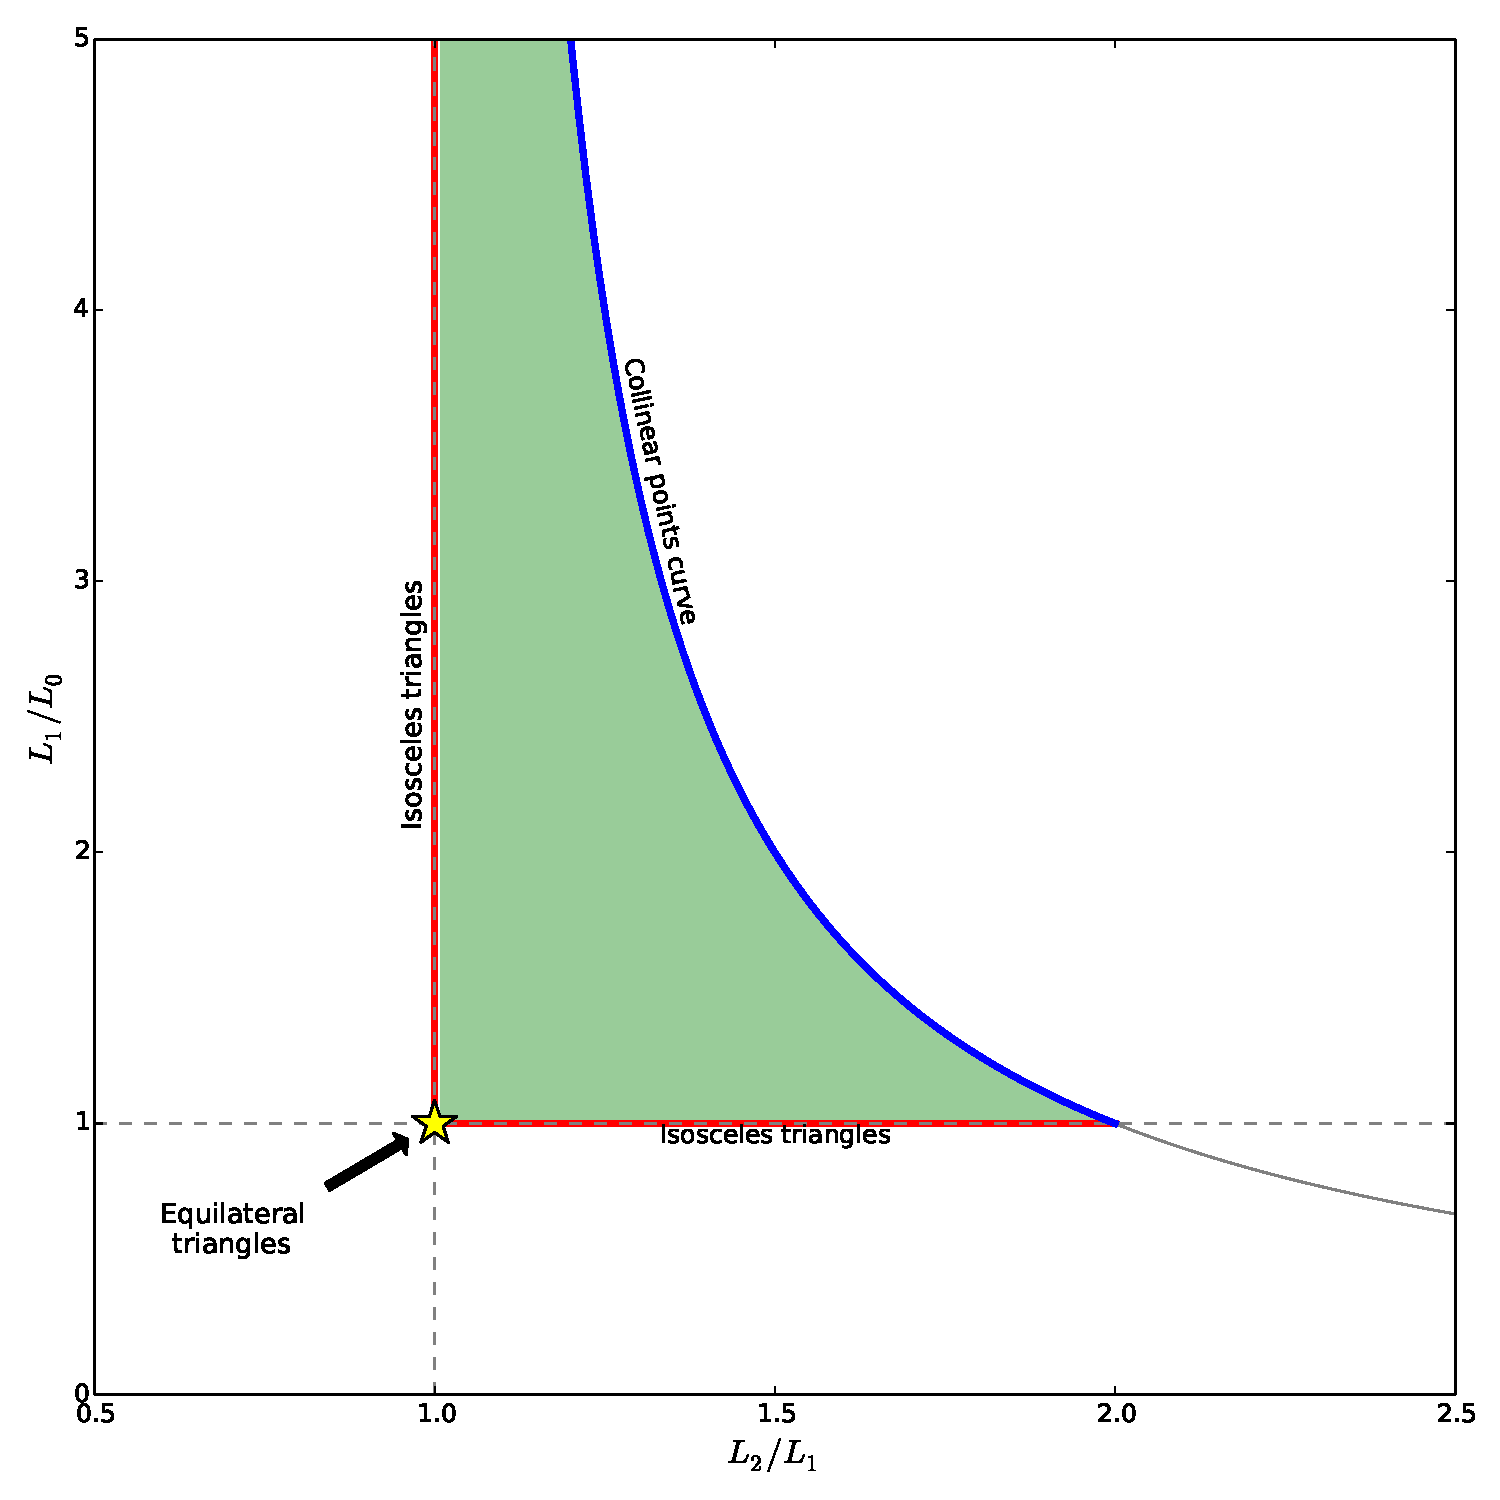
\includegraphics[width = \linewidth]{chapter_astroalign/figures/invariantMap01.pdf}
   \caption{Region for a particular invariant mapping}
   \label{fig:inv_region}
\end{figure}


%Other invariant sets can be constructed, each with a particular mapping from the set of side lengths of triangles to a region in the 2D plane of invariants.

%Some other examples are given in figure \ref{fig:inv_maps}. These have been explored numerically plotting the invariants for a large number of triangles.

%\begin{figure}[htb]
%   \centering
%   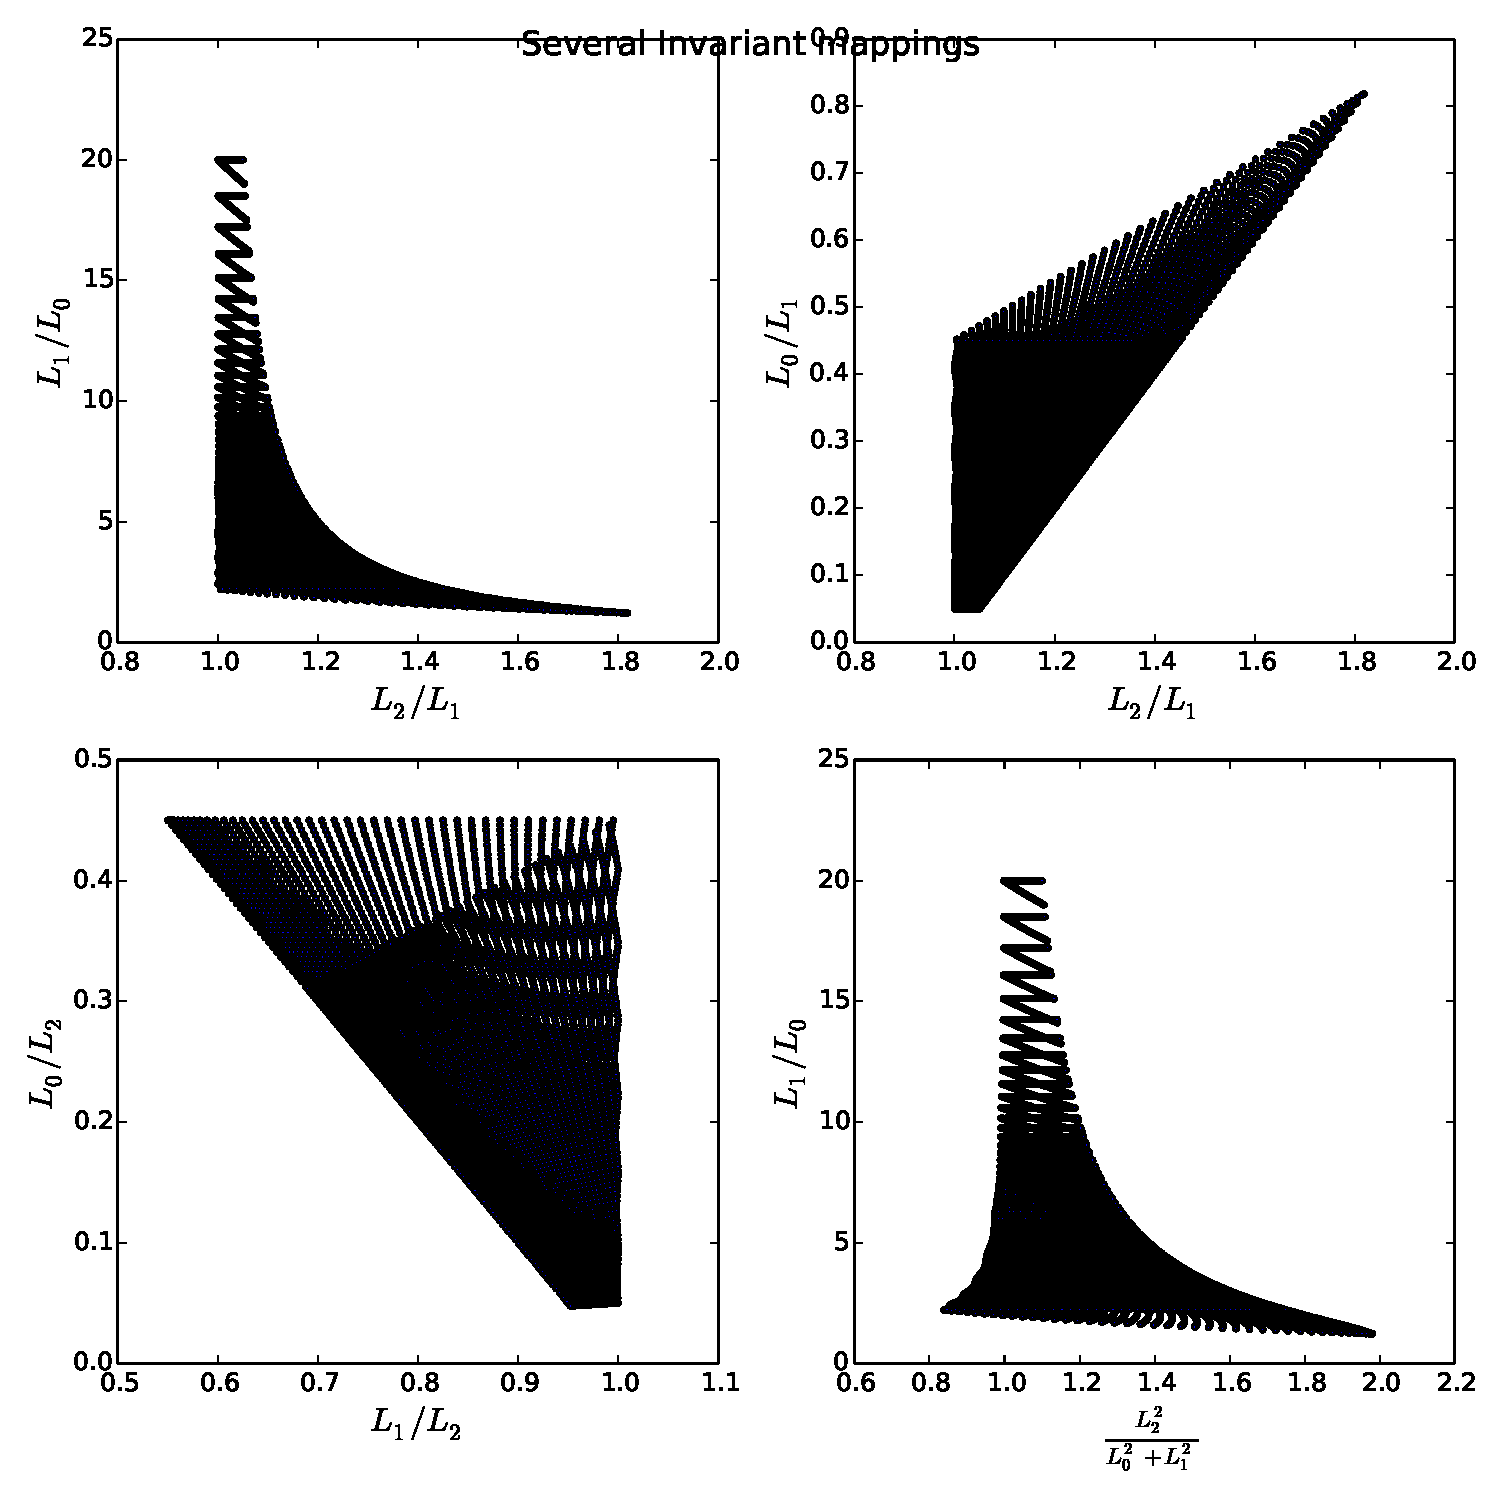
\includegraphics[width = \linewidth]{chapter_astroalign/figures/differentInvariantMaps.pdf}
%   \caption{Four examples of invariant mappings}
%   \label{fig:inv_maps}
%\end{figure}

%\lipsum

\subsection{An Ideal Example}

Let's see how the algorithm performs on an ideal example.

For this, we create several stars at random positions and we rotate and translate them as seen in figure \ref{fig:ideal_sources}.

\begin{figure}[htbp]
   \centering
   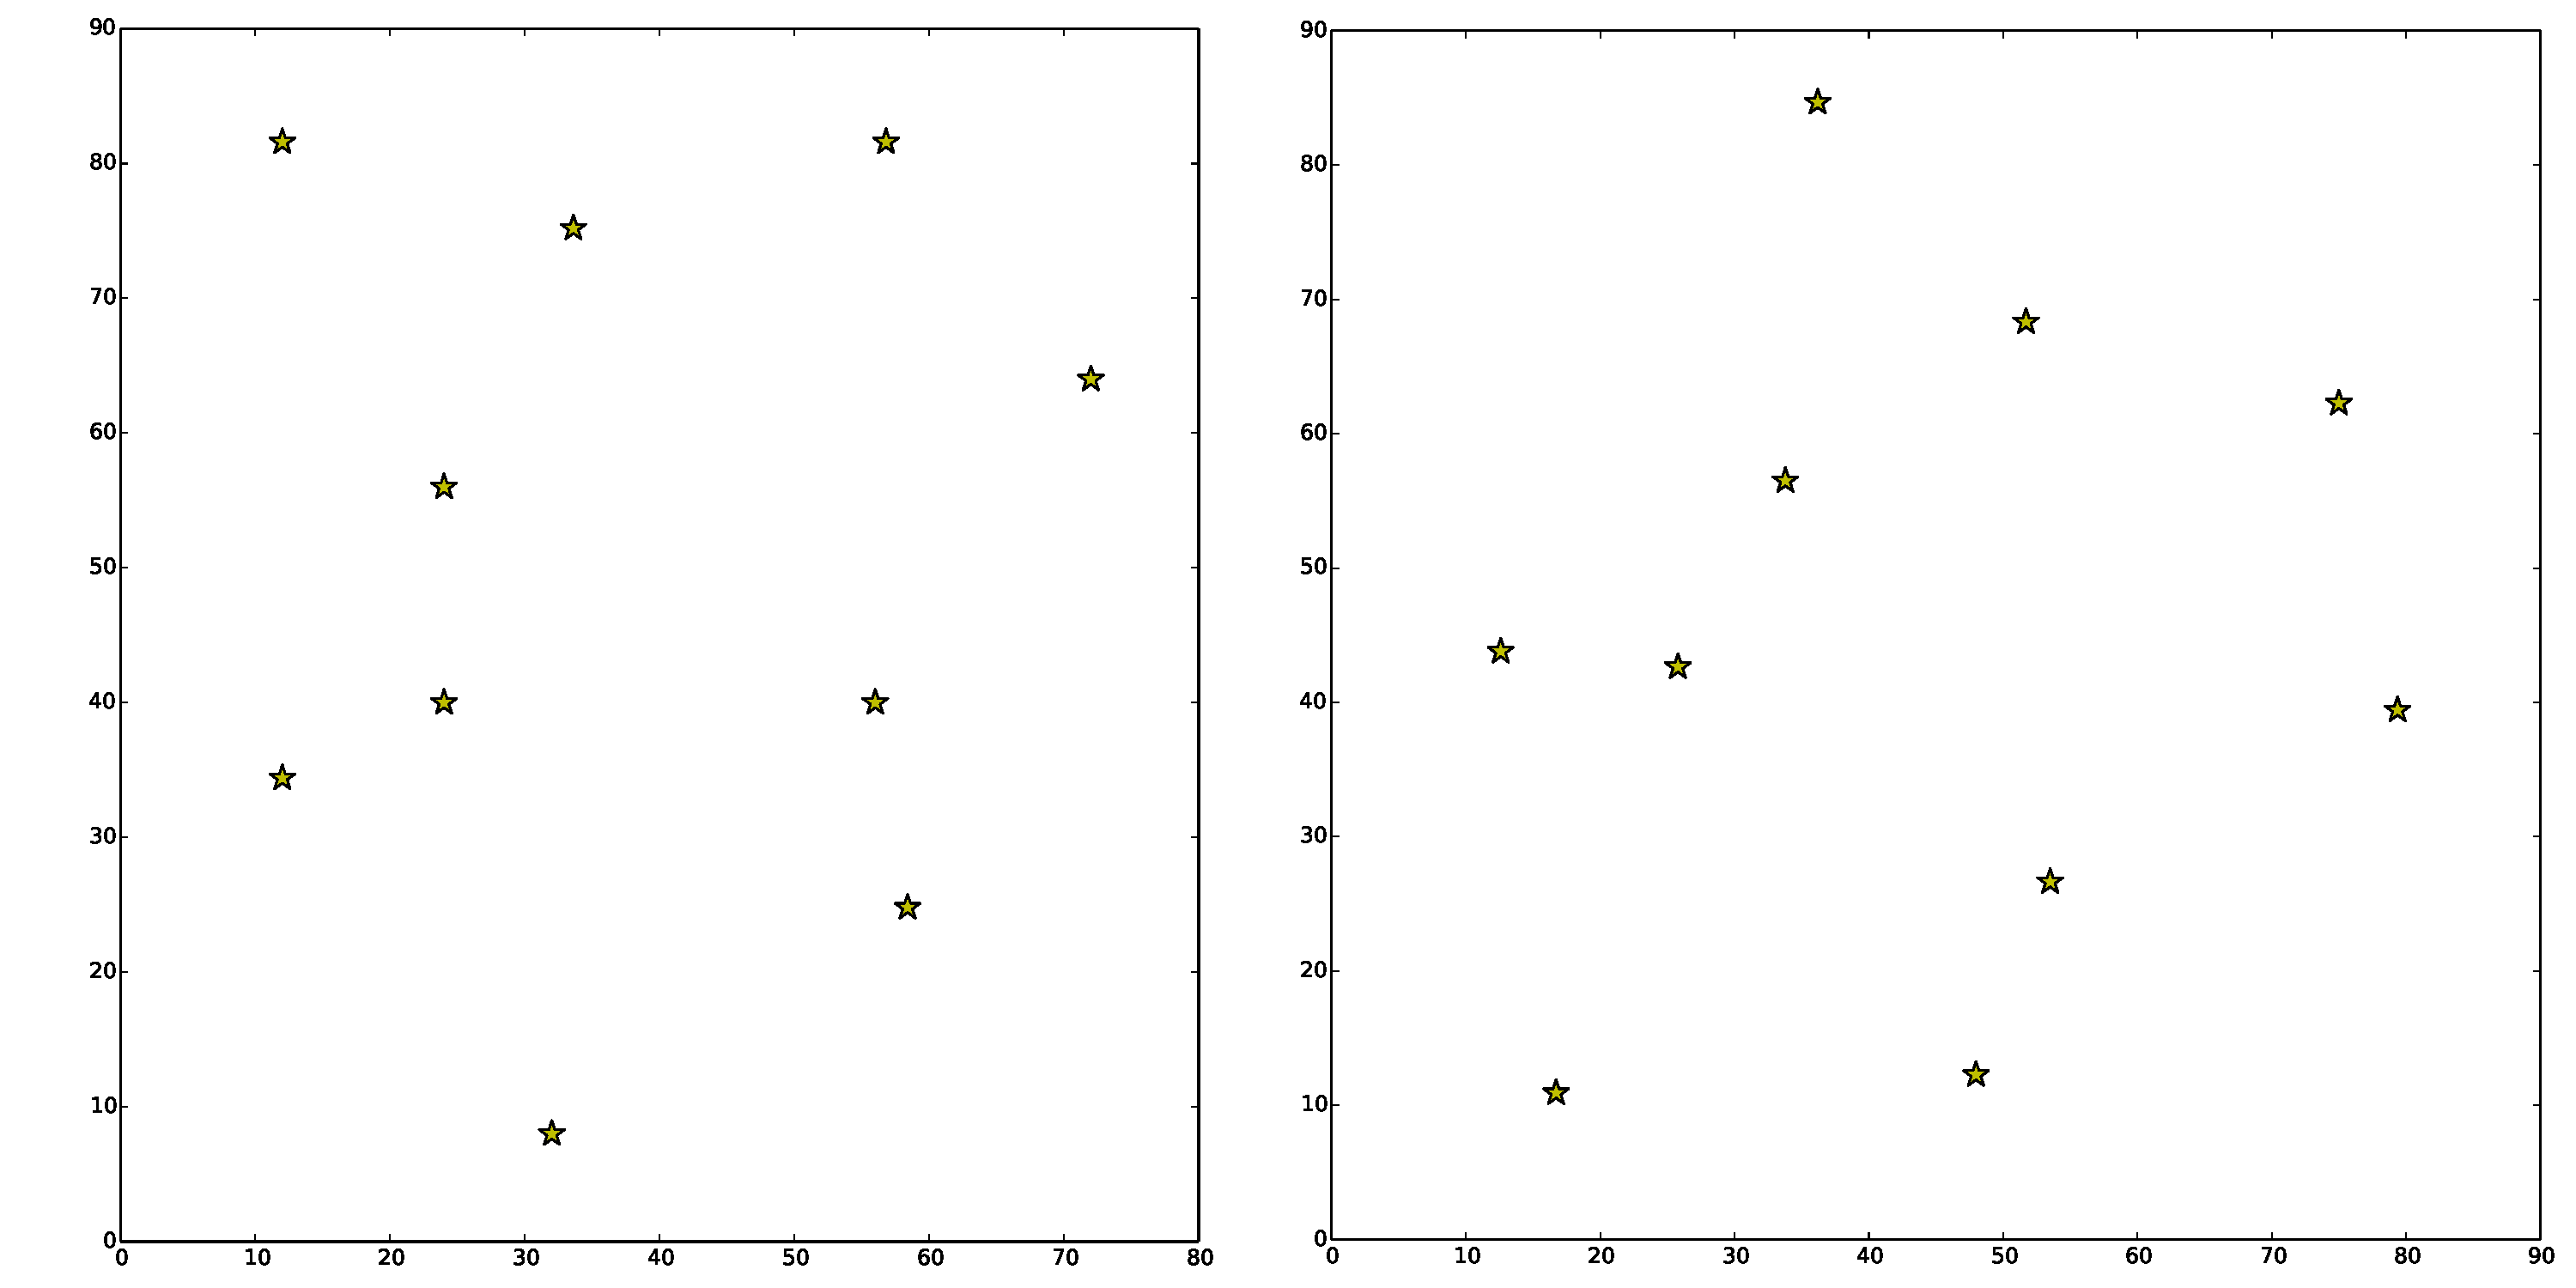
\includegraphics[width = \linewidth]{chapter_astroalign/figures/idealSources.pdf}
   \caption{Two ideal distribution of sources}
   \label{fig:ideal_sources}
\end{figure}

The invariant features in (\ref{inv01}) from this set of stars is plotted in figure \ref{fig:ideal_inv}.

\begin{figure}
   \centering
   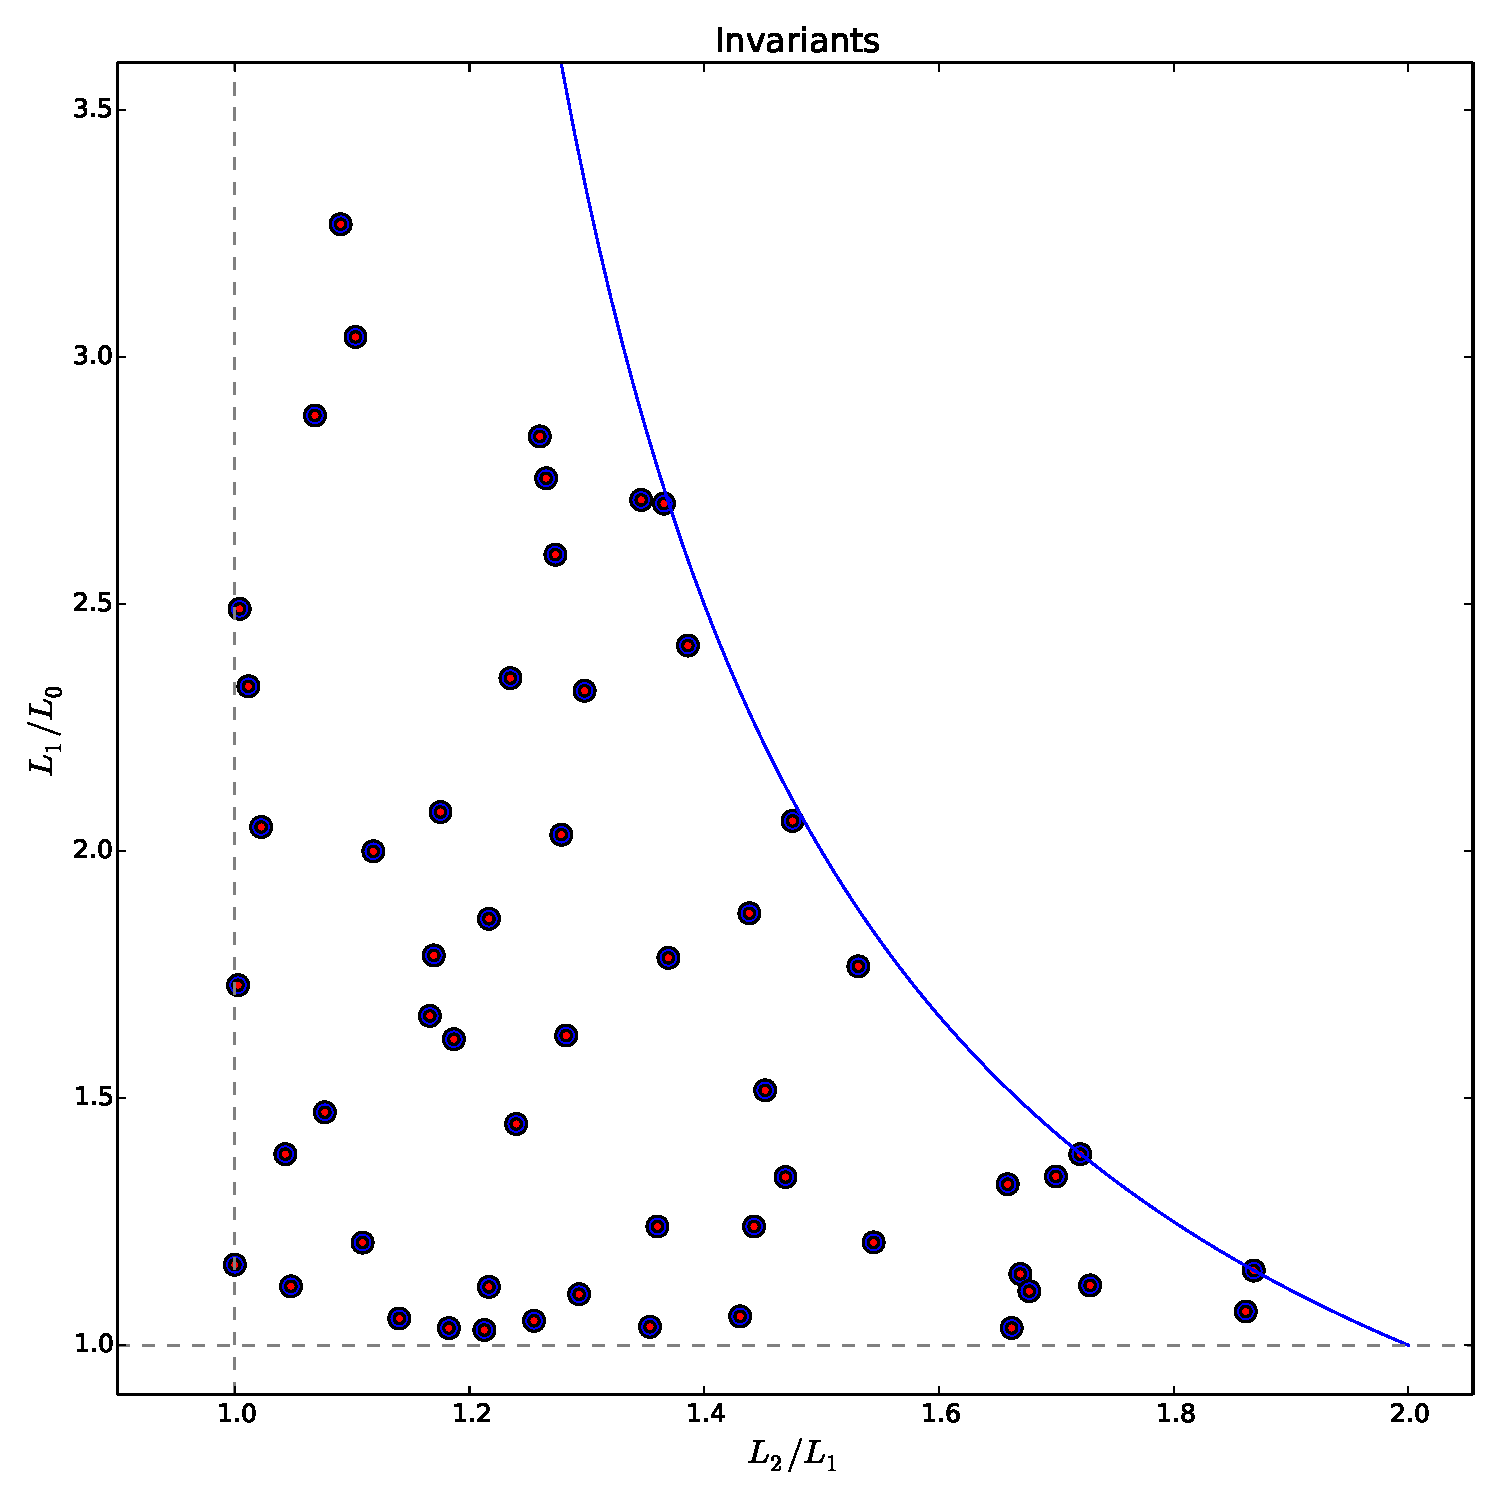
\includegraphics[width = \linewidth]{chapter_astroalign/figures/idealInvariants.pdf}
   \caption{Invariants for the ideal example}
   \label{fig:ideal_inv}
\end{figure}

We note that some invariants belong to collinear points, and the distribution of points is fairly sparse. 
This will help the identification phase when we try to match our triangles.

In the figure, the invariant points for both images were plotted. They appear superimposed in the plot.

We note that every blue invariant point has its corresponding red invariant point on top. 
There are no points without a partner for neither of the images. 
This is because all the sources in one image appear in the other one, there are no missing stars.
In a real situation, some stars will be missing because they are out of the field of view or because they became too faint due to extinction or any other technical reason. 
The algorithm should still work with missing or extra stars in the reference or test image. 

Another issue with real images is that locating the position of a source is not entirely precise, so small errors will appear in the expected position of one source with respect to its partner in the other image.
This error in turn creates an error on the lengths of the sides of the triangle and thus on the invariants calculated from it.
In practice, the invariant points will lay close to each other to a given small tolerance.

Once we have the set of invariants from both images, we query a correspondence to the kd-tree for possible matches within a given tolerance radius. 
Each returned match will be a correspondence between a triangle in one image and another. 
From each, we can make the point to point correspondence, provided all sides are unequal, and this will determine a unique transformation between the images.

Some of the correspondences won't be real ones. It could be that by chance there are two similar triangles in the images that belong to different set of stars.

This is where the RANSAC algorithm comes in.

\subsection{The RANSAC algorithm}

From its Wikipedia page 

{\em ``The Random sample consensus (RANSAC) algorithm is an iterative method to estimate parameters of a mathematical model from a set of observed data which contains outliers.''}

In our case the mathematical model is the similarity transformation between both images and the parameters are those of the transformation, i.e. the rotation, translation and uniform scaling parameters.

RANSAC is capable of choosing a transformation that fits most of the other triangles and is not affected by the rest of spurious outliers. 

This algorithm is also used in the computer vision package OpenCV for a very similar purpose, to ignore outliers when trying to estimate an homography between two images. 

In our case we look for the parameters $t_x$, $t_y$ for the translation in the $x$ and $y$ direction, the rotation angle $\alpha$ and the dilation parameter $\lambda$.

The transformation applied to a point $(x,y)$ will look like this:

\begin{align*}
\left(
 \begin{array}{lll} 
 \lambda \cos \alpha & \lambda \sin \alpha& \lambda t_x \\
 - \lambda \sin \alpha & \lambda \cos \alpha& \lambda t_y \\
 0 & 0 & 1
 \end{array}
\right)
\equiv
\left(
 \begin{array}{lll} 
 a_0 & b_0 & c_0 \\
-b_0 & a_0 & c_1 \\
 0 & 0 & 1
 \end{array}
\right)
\end{align*}

To make our problem linear, we will consider the parameters $a_0, b_0, c_0, c_1$ as if they were independent.

Two data points pairs are sufficient to determine uniquely a transformation for this 4 parameters. 
More can be used if we use a linear square minimization.

%This candidate transformation $T$ will be tested against all the other triangle matches in a RANSAC algorithm.

\subsection{Error propagation}

Doing a simple propagation of errors we see that for nearly equilateral triangles $L_{1} \approx L_{2} \approx L_{3} \approx L$, 
the errors in the invariants go like $\Delta I_{i} \sim \frac{\Delta L}{L}$.
This means that, for invariants near $(I_{1}, I_{2}) = (1, 1)$ errors in the determination of the lengths of the triangle side will not magnify errors in the invariants.

%This is done by \citet{1995PASP..107.1119V}.
